\subsection{Scenario setup} \label{sec:lv_scenario_setup}
In this experiment, we placed different sensors in the network. The sensors have a limited sensing range, which means that they are only able to observe a portion of the total traffic. We have studied the independence of the samples gathered by the sensors in order to know if it is possible to use the semi-Markovian model proposed for the Local View model.

We used two different user realizations and number of sensors. This is represented in Figures \ref{fig:autocorrelation_lv_8sessions} and \ref{fig:autocorrelation_lv_15sessions}.

\begin{figure}[h!]
	\centering
	\subfloat[8 sessions]{
		\includegraphics[width=0.5\textwidth, trim = 0mm 0mm 0mm 0mm, clip]{images/results/autocorrelation/localview/8sessions}
		\label{fig:autocorrelation_lv_8sessions}
	}
	\subfloat[15 sessions]{
		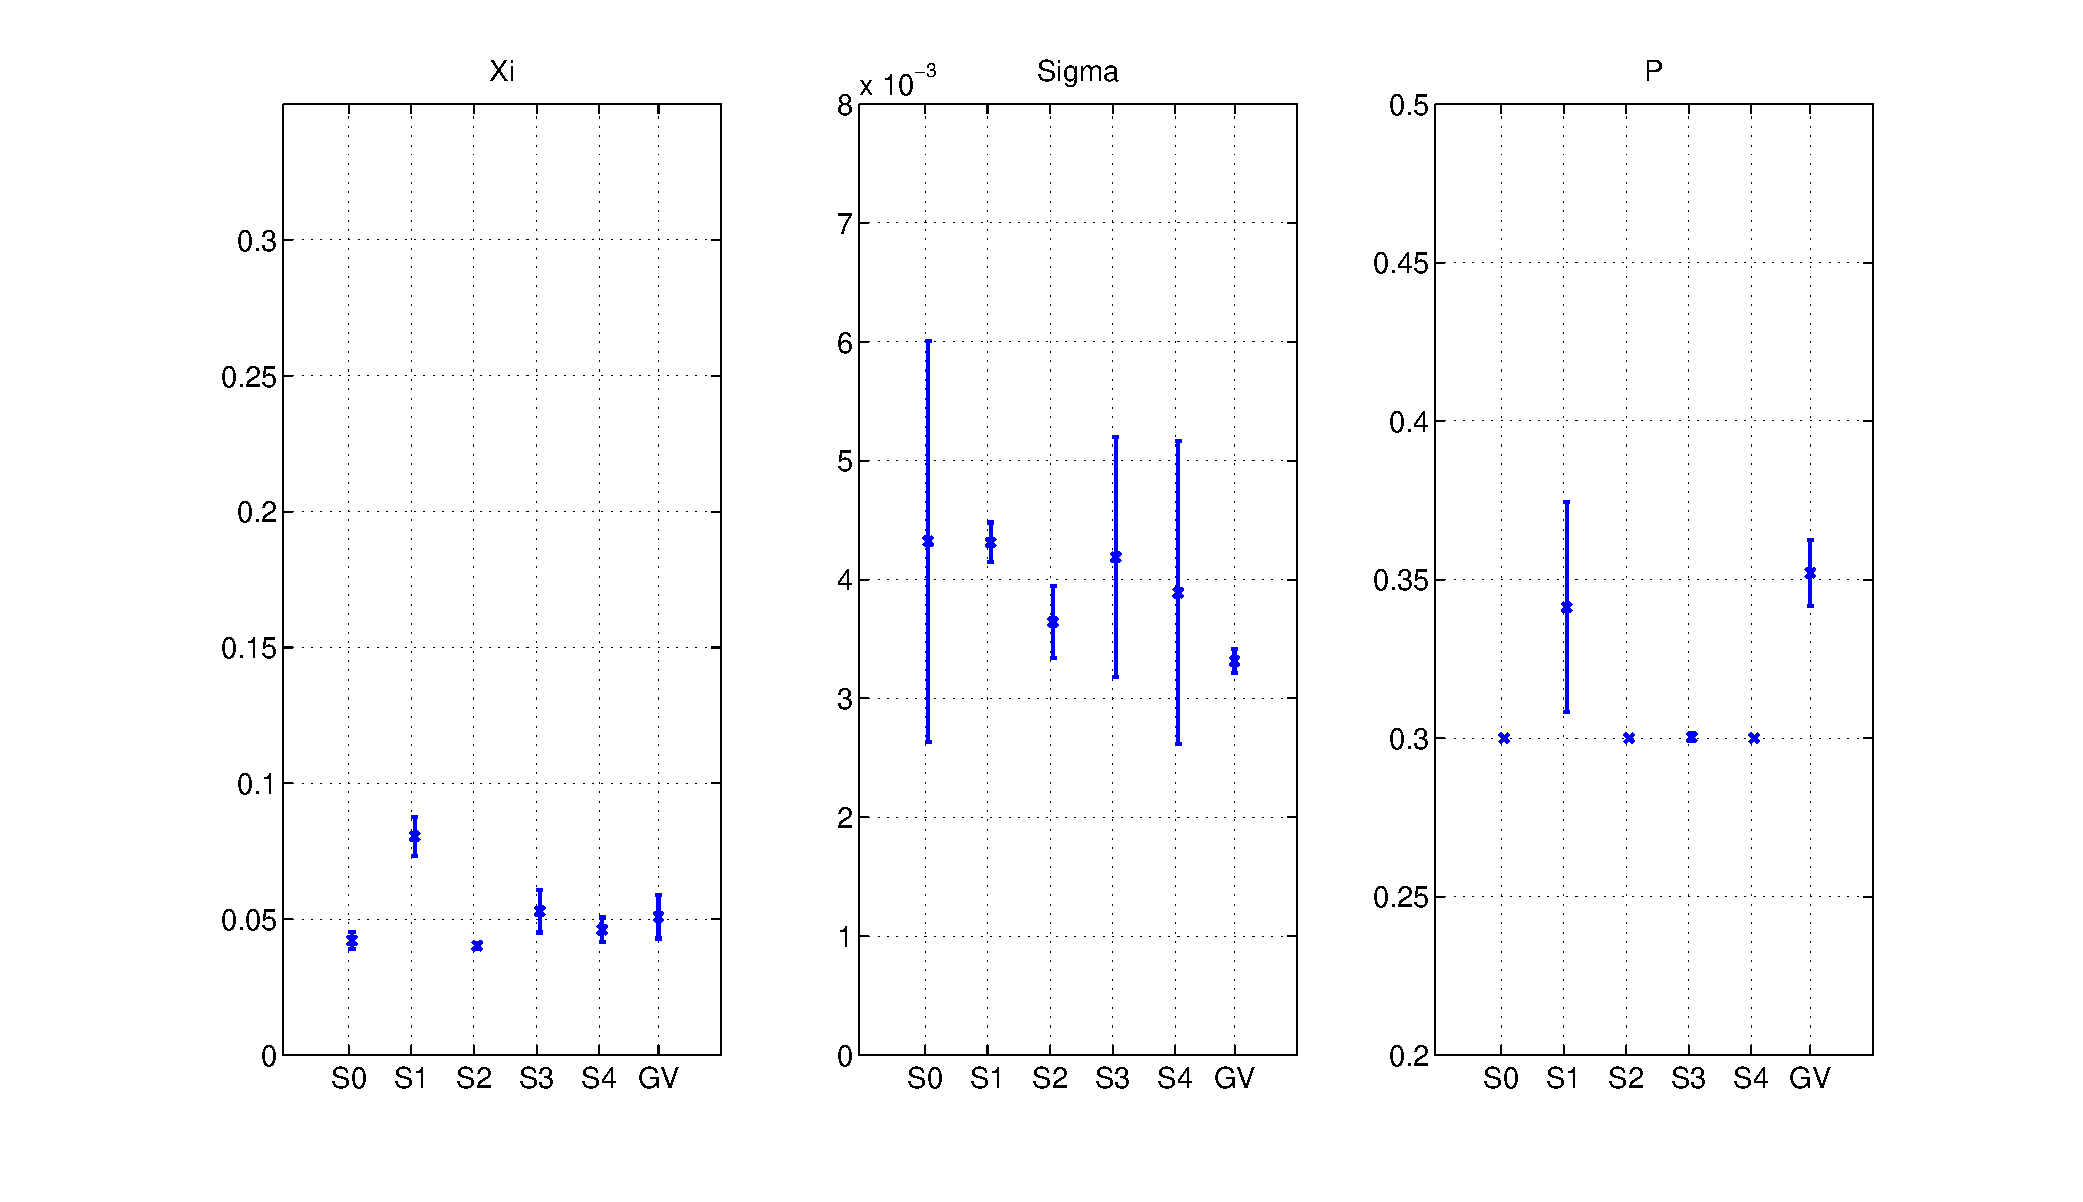
\includegraphics[width=0.5\textwidth, trim = 0mm 0mm 0mm 0mm, clip]{images/results/autocorrelation/localview/15sessions}
		\label{fig:autocorrelation_lv_15sessions}
	}
	\caption{User realizations for the Local View autocorrelation experiments (examples)}
	\label{fig:autocorrelation_lv_users}
\end{figure}

As it can be observed, each one of the sensors observe a different amount of \acs{WLAN} users. This will give us the opportunity to study how different number of sessions and load affect the correlation of the active periods gathered by each one of the sensors. We did not performed the estimation process for this experiments.

\subsection{Autocorrelation of the IN/OUT sequence of DATA packets in Local View - Results} \label{sec:autocorrelation_lv_results}
From the simulation trace files, we obtain the sequence of active periods and which \acs{WLAN} stations are generating these periods. In order to study the autocorrelation of the samples, we obtained which \acs{WLAN} stations are observed by each one of the sensors and, from the stations sequence obtained from the simulation's trace file, we generated a IN/OUT sequence depending on whether the stations are observed by the sensor or not. We finally obtained the autocorrelation function of this IN/OUT sequence. The results are presented in Figure \ref{fig:autocorrelation_lv_8sessions_sensors} and \ref{fig:autocorrelation_lv_15sessions_sensors}.

\begin{figure}[h!]
	\centering
	\subfloat[Sensor 0 - Obs: 2 sessions]{
		\includegraphics[width=0.33\textwidth, trim = 0mm 0mm 0mm 0mm, clip]{images/results/autocorrelation/localview/8sessions_sensor0}
		\label{fig:autocorrelation_lv_8sessions_s0}
	}
	\subfloat[Sensor 1 - Obs: 4 sessions]{
		\includegraphics[width=0.33\textwidth, trim = 0mm 0mm 0mm 0mm, clip]{images/results/autocorrelation/localview/8sessions_sensor1}
		\label{fig:autocorrelation_lv_8sessions_s1}
	}
	\subfloat[Sensor 2 - Obs: 2 sessions]{
		\includegraphics[width=0.33\textwidth, trim = 0mm 0mm 0mm 0mm, clip]{images/results/autocorrelation/localview/8sessions_sensor2}
		\label{fig:autocorrelation_lv_8sessions_s2}
	}
	\caption{Autocorrelation of the IN/OUT sequences for 8 sessions.}
	\label{fig:autocorrelation_lv_8sessions_sensors}
\end{figure}

\begin{figure}[h!]
	\centering
	\subfloat[Sensor 0 - Obs: 5 sessions]{
		\includegraphics[width=0.33\textwidth, trim = 0mm 0mm 0mm 0mm, clip]{images/results/autocorrelation/localview/15sessions_sensor0}
		\label{fig:autocorrelation_lv_15sessions_s0}
	}
	\subfloat[Sensor 1 - Obs: 7 sessions]{
		\includegraphics[width=0.33\textwidth, trim = 0mm 0mm 0mm 0mm, clip]{images/results/autocorrelation/localview/15sessions_sensor1}
		\label{fig:autocorrelation_lv_15sessions_s1}
	}
	\subfloat[Sensor 2 - Obs: 3 sessions]{
		\includegraphics[width=0.33\textwidth, trim = 0mm 0mm 0mm 0mm, clip]{images/results/autocorrelation/localview/15sessions_sensor2}
		\label{fig:autocorrelation_lv_15sessions_s2}
	}
	\\
	\subfloat[Sensor 3 - Obs: 8 sessions]{
		\includegraphics[width=0.33\textwidth, trim = 0mm 0mm 0mm 0mm, clip]{images/results/autocorrelation/localview/15sessions_sensor3}
		\label{fig:autocorrelation_lv_15sessions_s3}
	}
	\subfloat[Sensor 4 - Obs: 8 sessions]{
		\includegraphics[width=0.33\textwidth, trim = 0mm 0mm 0mm 0mm, clip]{images/results/autocorrelation/localview/15sessions_sensor4}
		\label{fig:autocorrelation_lv_15sessions_s4}
	}
	\caption{Autocorrelation of the IN/OUT sequences for 15 sessions.}
	\label{fig:autocorrelation_lv_15sessions_sensors}
\end{figure}

As it can be observed in the 8-session case, the autocorrelation property of the sequence for the two of the sensors (0 and 2) can be considered good: the harmonics are almost negligible and the function is approximated to a $\delta$. This means that the samples in this case are independent and this case is a good candidate in order to apply the Local View model since the assumption of independence of the active periods holds. It can be observed how the autocorrelation function in Sensor 1 is slightly worst.

For those cases in which the sequence of consecutive active periods is non-correlated (Sensors 0 and 2 in the 8-session case, for example), the Local View model can be applied properly since the assumption of correlation holds. However, we are facing an important problem: if the sensors need to study the correlation of consecutive active periods from the IN/OUT sequence in order to determine if the Local View can be applied, they need to have knowledge of how is the spectrum activity outside the sensor's range, which means that the sensors need to have a Global View capability or cooperate with other sensors in the \acs{WSN} in order to determine this IN/OUT sequence.

\subsection{Density study of the consecutive skipped Active periods in Local View - Results} \label{sec:autocorrelation_lv_skipped_results}
In extension to the autocorrelation study of the active periods in Section \ref{sec:autocorrelation_lv_results}, we will study the correlation of consecutive skipped active periods using the autocorrelation function. For this, we will construct a sequence of number of consecutive active periods that the sensors are unable to observe because of \acs{WLAN} users outside sensing range.

The traffic of the network is formed by a sequence of active-idle periods generated by the different users. A sensor with a limited sensing range will only observe a portion of this traffic, generated by the users within its sensing range. Therefore, the sensor will 'miss' some of the active periods that are generated by users outside its sensing range. Using the same users realizations used in Section \ref{sec:autocorrelation_lv_results}, we will extract the sequence of the consecutive skipped active periods and perform an autocorrelation study in order to observe its behavior.

From the first results obtained in this experiment, we observed that the sequence consecutive active periods follow a Geometric Distribution. The geometric distribution is a memory-less distribution and is characterized by a single parameter: $p$. This parameter can be obtained from the mean value of the samples. For this, we obtain the mean value of the sequence of consecutive skipped active periods of each sensor and obtain the $p$ value by:

\begin{equation}
	p = \frac{1}{1+E(x)}
	\label{eq:p_geometric}
\end{equation}

With this parameter we will construct a geometric distribution and we will test its fitting with the empirical distribution from the samples. The CDF of the geometric distribution can be found with:

\begin{equation}
	CDF(k) = 1 - (1 - p)^{k+1} 
	\label{eq:geometric_cdf}
\end{equation}

The results obtained from this experiment can be observed in Figures \ref{fig:8sessions_geometric} and \ref{fig:15sessions_geometric}. The user realizations and number of sensors are represented in Figure \ref{fig:autocorrelation_lv_users}.

\begin{figure}[h!]
	\centering
	\subfloat[Sensor 0: Observes 2 users]{
		\label{fig:8sessions_sensor0}
		\includegraphics[width=\textwidth]{images/results/autocorrelation/localview/fitting/8sessions_sensor0}
	}%\\
	%\subfloat[Sensor 1: Observes 4 users]{
	%	\label{fig:8sessions_sensor0}
	%	\includegraphics[width=\textwidth]{images/results/autocorrelation/localview/fitting/8sessions_sensor1}
	%}\\
	%\subfloat[Sensor 2: Observes 2 users]{
	%	\label{fig:8sessions_sensor0}
	%	\includegraphics[width=\textwidth]{images/results/autocorrelation/localview/fitting/8sessions_sensor2}
	%}
	\caption{8 sessions - Example of fitting of the geometric distribution and autocorrelation of the IN/OUT sequence + consecutive skipped active periods}
	\label{fig:8sessions_geometric}
\end{figure}

\begin{figure}[h!]
	\centering
	%\subfloat[Sensor 0: Observes 5 users]{
	%	\label{fig:15sessions_sensor0}
	%	\includegraphics[height=0.18\textheight]{images/results/autocorrelation/localview/fitting/15sessions_sensor0}
	%}\\
	%\subfloat[Sensor 1: Observes 7 users]{
	%	\label{fig:15sessions_sensor0}
	%	\includegraphics[height=0.18\textheight]{images/results/autocorrelation/localview/fitting/15sessions_sensor1}
	%}\\
	%\subfloat[Sensor 2: Observes 3 users]{
	%	\label{fig:15sessions_sensor0}
	%	\includegraphics[height=0.18\textheight]{images/results/autocorrelation/localview/fitting/15sessions_sensor2}
	%}\\
	%\subfloat[Sensor 3: Observes 8 users]{
	%	\label{fig:15sessions_sensor0}
	%	\includegraphics[height=0.18\textheight]{images/results/autocorrelation/localview/fitting/15sessions_sensor3}
	%}\\
	\subfloat[Sensor 4: Observes 8 users]{
		\label{fig:15sessions_sensor0}
		\includegraphics[width=\textwidth]{images/results/autocorrelation/localview/fitting/15sessions_sensor4}
	}
	\caption{15 sessions - Example of fitting of the geometric distribution and autocorrelation of the IN/OUT sequence + consecutive skipped active periods}
	\label{fig:15sessions_geometric}
\end{figure}

As it can be observed from Figures \ref{fig:8sessions_geometric} and \ref{fig:15sessions_geometric}, we have represented the autocorrelation function of the IN/OUT sequence for the sensor (see Section \ref{sec:autocorrelation_lv_results}), the fitting of the empirical and geometric distributions, and the autocorrelation function of the sequence of consecutive skipped active periods. From the autocorrelation function of the skipped samples we can say that there is independence between consecutive skipped samples, which was already expected from the results presented previously. In addition, we also represented the fitting of the CDF of the skipped samples and its approximation using the Geometric Distribution. As it can be observed from this fitting, it can be said that the geometric function is a good candidate in order to model the consecutive skipped samples for the Local View model.

\subsubsection{Goodness-of-fit test for the consecutive skipped active periods} \label{sec:gof_lv_skipped}
As it has been done in previous sections, the fitting can be tested using a Goodness-of-fit test. In this case, the Kolmogorov-Smirnov test cannot be used. The \acs{K-S} test requires the samples to be independent and follow a continuous behavior. Our sequence of skipped samples follow is represented by a discrete distribution. For this, the \acs{K-S} cannot be used to test the fitting of the geometric distribution against our empirical data.

First we studied a modification of the Kolmogorov-Smirnov test for discrete distributions \cite{ks_discrete}, but it was not the easiest solution to implement. We proposed and tested two different solutions to test the fitting which were more easy to implement with the available data: Mean Square Error test and Chi-squared Goodness-of-fit test.

The Mean Square Error (\acs{MSE}) is based on testing the deviation between both distributions (empirical and geometric) and obtaining the mean square error using the expression (\ref{eq:MSE}), where $N$ determines the number of samples for the validation test and $k$ is the $k_th$ sample.

\begin{equation}
	\sum_{k=0}^{N}[P_{geometric}(k) - P_{empirical}(k)]^2
	\label{eq:MSE}
\end{equation}


For this test, we run 100 times the same simulation configuration and extracted the \acs{MSE} between both distributions for each run. The results are represented in Figure \ref{fig:mse_cdf} in which we have represented the CDF of the MSE for the 100 runs.

On the other hand, we also tested the fitness of the empirical and geometric distributions using the Goodness-of-fit test Chi-squared. This test can be applied for both continuous and discrete distributions. For this test we also run 100 times the same simulation configuration and extracted the CDF of the p-value. The Chi-square test has been obtained using the already implemented function in MATLAB. The results are presented in Figure \ref{fig:chi2_cdf}.

For the Chi-square test, as it is done in the Kolmogorov-Smirnov, the confidence limit to reject the null hypothesis is $0.1$. In this case, we can observe that there is a high percentage of the 100 runs that the null hypothesis is rejected. In order to know if this failure rate is because of the MATLAB implementation of the Chi-square test which can be to restrictive or because of bad fitting, we plotted the fitting of the empirical and geometric distribution for a high and low p-value of the validation test. This is represented in Figure \ref{fig:chi2_bad_good}.

As it can be observed in Figure \ref{fig:bad_p1}, where the p-value of the validation test is really low, the fitting between both distributions is clearly bad and in extension the validation test is failing. On the other hand, Figure \ref{fig:good_p} represents one of the best p-value cases for one of the sensors and it can be observed how the fitting between distributions is almost perfect. However, this behavior was also present in those fail cases in which the p-value was close to the confidence limit $p<0.1$. The high failure rate of the Chi-squared test may be caused because the implementation in MATLAB is too restrictive and the minimum deviation between distributions affects highly the final p-value. A further study in this topic is needed.

\begin{figure}[h!]
	\centering
	\subfloat[8 sessions]{
		%\label{fig:8sessions_sensor0}
		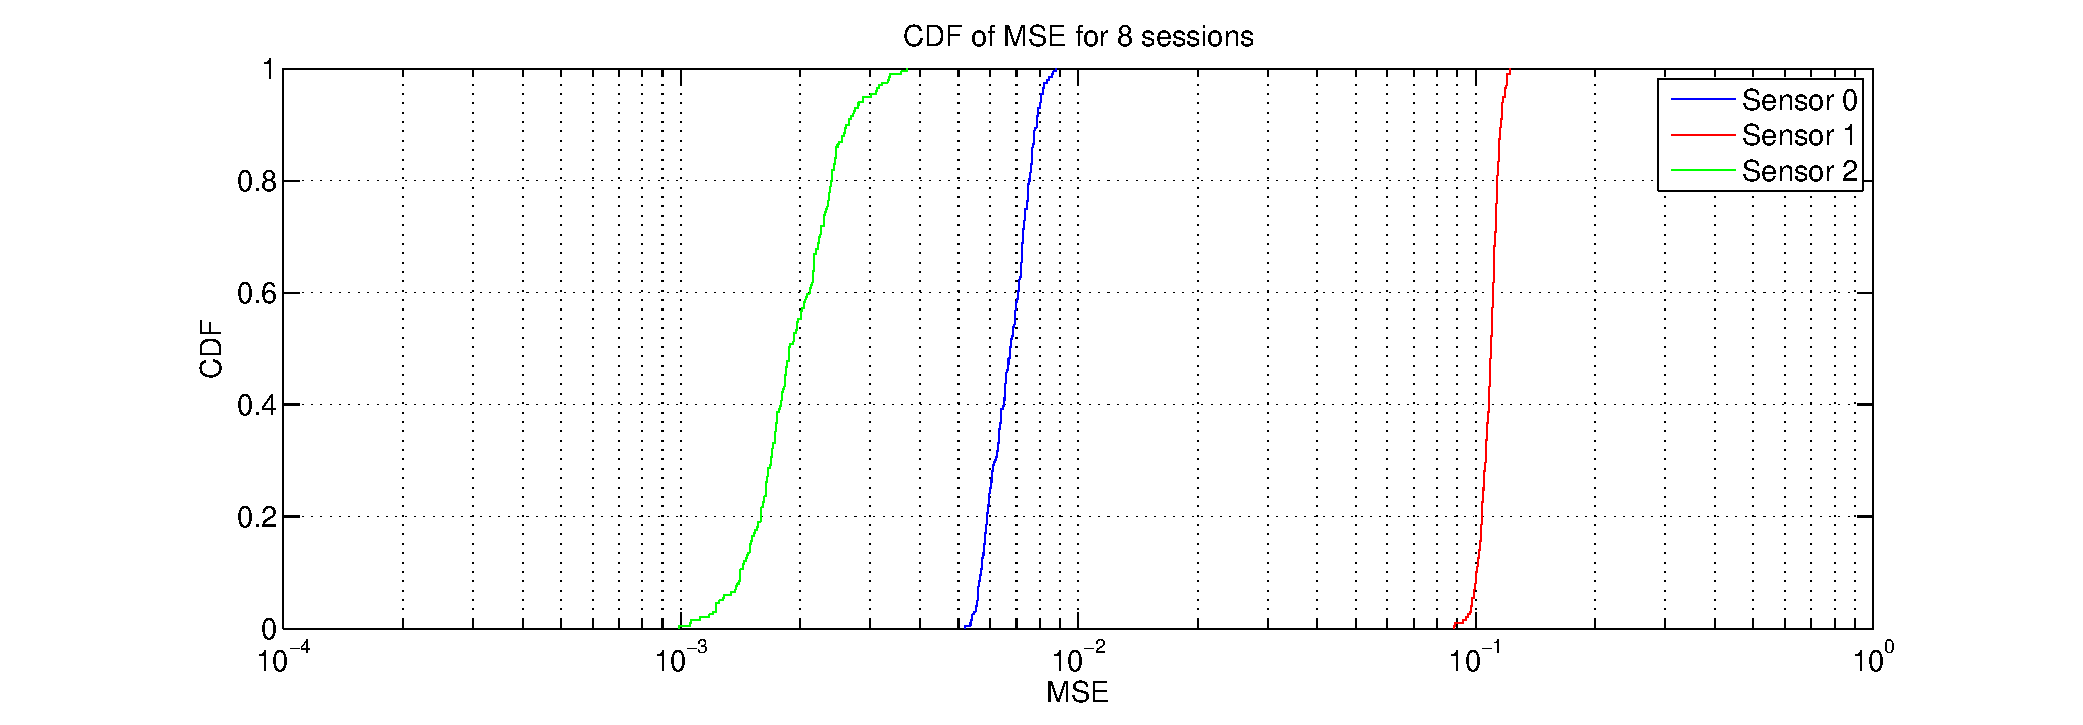
\includegraphics[width=1\textwidth]{images/results/autocorrelation/localview/mse/8sessions_MSE}
	}\\
	\subfloat[15 sessions]{
		%\label{fig:8sessions_sensor0}
		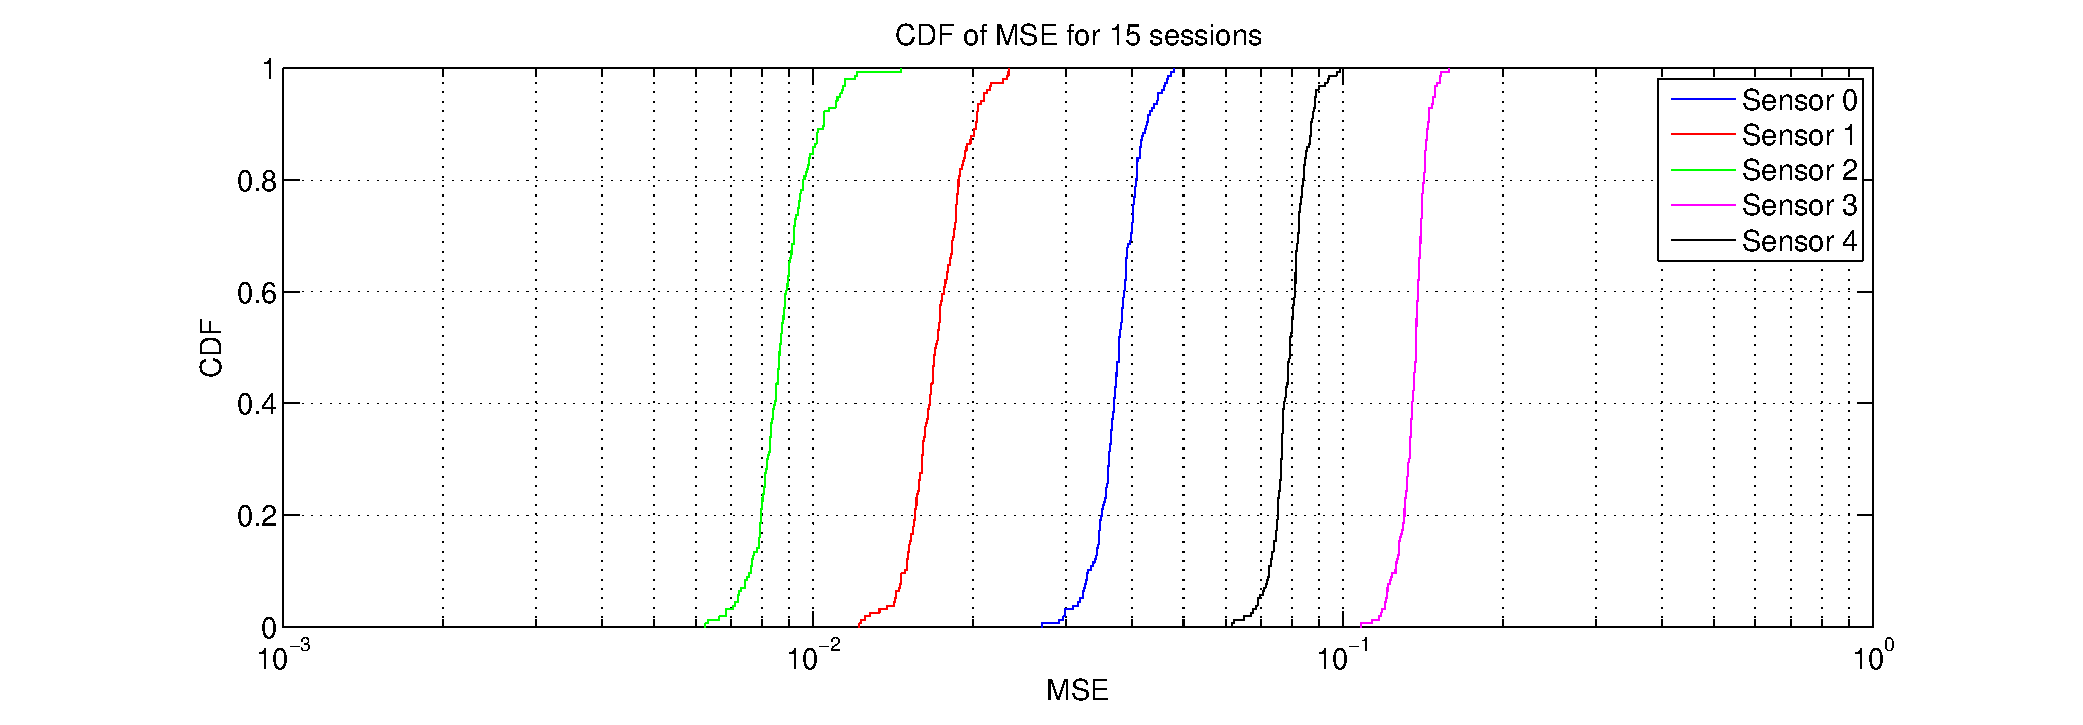
\includegraphics[width=1\textwidth]{images/results/autocorrelation/localview/mse/15sessions_MSE}
	}
	\caption{CDF of the MSE for different sensors}
	\label{fig:mse_cdf}
\end{figure}

\begin{figure}[h!]
	\centering
	\subfloat[]{
		\label{fig:8sessions_chi2_p}
		\includegraphics[width=0.5\textwidth]{images/results/autocorrelation/localview/chi2/8sessions_cdf_p}
	}
	\subfloat[]{
		\label{fig:15sessions_chi2_p}
		\includegraphics[width=0.5\textwidth]{images/results/autocorrelation/localview/chi2/15sessions_cdf_p}
	}
	\caption{CDF of the p-value using the Chi-square Goodness-of-fit test}
	\label{fig:chi2_cdf}
\end{figure}

\begin{figure}[h!]
	\centering
	\subfloat[]{
		\label{fig:bad_p1}
		\includegraphics[width=0.50\textwidth]{images/results/autocorrelation/localview/chi2/8sessions_sensor2_badpvalue}
	}
	\subfloat[]{
		\label{fig:good_p}
		\includegraphics[width=0.50\textwidth]{images/results/autocorrelation/localview/chi2/8sessions_sensor0_goodpvalue}
	}
	\caption{Fitting of the empirical and geometric distributions for different p-values}
	\label{fig:chi2_bad_good}
\end{figure}